% This work is the property of Aleksandr Salo,
% Student of Baylor University, Computer Science Department. 
% Copying or using without notifying me is not allowed. 
% Contact email is alexsalovrn@gmail.com

\documentclass{article}

\usepackage{fullpage}
\usepackage{url}
\usepackage{hyperref}
\usepackage{amssymb}
\usepackage{amsmath}
\usepackage{graphicx}
\usepackage{epstopdf}
\usepackage{epsfig}
\usepackage{caption}
\usepackage{subcaption}
\usepackage[]{mcode}
\usepackage{listings}
\usepackage{dsfont}
\lstset{language=Python}


\newcommand*{\Perm}[2]{{}^{#1}\!P_{#2}}%
\newcommand*{\Comb}[2]{{}^{#1}C_{#2}}%
\newcommand{\mytilde}{\raise.17ex\hbox{$\scriptstyle\mathtt{\sim}$}}
\newcommand{\patheta}{\frac{\partial}{\partial \theta_j} }
\newcommand{\pathe}{\frac{\partial}{\partial \theta} }
\newcommand{\pathx}{\frac{\partial}{\partial X} }
\newcommand{\thetax}{\theta^T x}
\newcommand{\elll}{\ell(\theta)}
\newcommand{\nath}{\nabla_\theta}
\newcommand{\pelll}{\frac{\partial^2 \elll}{\partial \theta_j \partial \theta_k}}
\newcommand{\ith}{^{(i)}}
\newcommand{\jth}{^{(j)}}
\newcommand{\gdafrac}{\frac{1}{(2\pi)^{n/2}|\Sigma|^{1/2}}\exp}
\newcommand{\hhat}{\hat{h}}

% Dr. Hamerly's customization
% tell Latex to use no paragraph indentation, but leave some space between
% paragraphs 
\setlength{\parindent}{0in}
\setlength{\parskip}{0.1in}

\title{Assignment 3}
\date{Due April 9, 2015}
\author{Aleksandr Salo}

\begin{document}
\maketitle

\section{Uniform convergence (20 points)}
	\begin{enumerate}
		\item  We proved that for any finite set of hypotheses $H = \{h_1,...,h_k\}$, if we pick the hypothesis $\hat{h}$	that minimizes the training error on a set of m examples, then with probability at least $1-\delta$:
		$$ \epsilon (\hat{h}) \le (\min_i \epsilon(h_i)+2 \sqrt{\frac{1}{2m} log \frac{2k}{\delta}})$$
		
		Consider a learning algorithm which, after looking at m training examples, chooses some hypothesis
		$\hat{h} \in H$ that makes zero mistakes on this training data. This process may yield a hypothesis that makes no mistakes in training, but still has non-zero generalization error. Show that with probability ($1-\delta$):
		$$\epsilon (\hat{h}) \le \frac{1}{m} log \frac{k}{\delta}$$
		
		\textbf{Proof:}
		\begin{enumerate}
			\item Let $\hat{h}$ be a bad classifier, that doesn't generalize very well: 
			$$\epsilon(\hhat) > \gamma$$
			\item We may choose this classifier, if for given training set $S_m$ it has zero training error. The probability, that chosen classifier would \textbf{not} make an error on the one particular example is (by definition):
			$$P(\text{Correct decision}) \le 1 - \hat{\epsilon}(\hhat))$$			
			\item Then the probability that the classifier would \textbf{not} fail for all the examples in training set is:
			\begin{align*}
			P(\text{All correct}) &\le (1 - \hat{\epsilon}(\hhat))^m \\
			&\le  (1 - \gamma)^m \\
			& \le e^{-\gamma m} 
			\end{align*}
			
			\item Now let us think about all the such bad classifiers out there and apply union bound. The probability that all (k) of them would \textbf{not} fail on any training example is (by union bound):
			\begin{align*}
			P &= k(1 - \gamma)^m\\
			&\le ke^{-\gamma m}			
			\end{align*}
						
			We want that probability to be equal to $\delta$, so:
			$$ke^{-\gamma m}  = \delta$$
						
			\item Let solve for $\gamma$:
			\begin{align*}
			ke^{-\gamma m} &= \delta\\
			e^{-\gamma m} &= \frac{\delta}{k}\\
			-\gamma m &= \log \frac{\delta}{k}\\
			\gamma &= -\frac{1}{m}\log \frac{\delta}{k}\\
			\gamma &= \frac{1}{m}\log \frac{k}{\delta}\\
			\end{align*}
			
			\item Thus we showed that with probability $(1 - \delta)$:
			$$\epsilon(\hhat) \le \frac{1}{m}\log \frac{k}{\delta}\\$$			
		\end{enumerate}
		
		\item  Let us take us mid stage formula from part 1 for a spin: $ke^{-\gamma m}  = \delta$ and write the above bound in form of sample complexity bound:
		\begin{align*}
		-\gamma m &= \log \frac{\delta}{k}\\
		m &= -\frac{1}{\gamma}\frac{\delta}{k}\\
		m & = \frac{1}{\gamma}\log \frac{k}{\delta}
		\end{align*}
		Thus, for m bigger than this, $\epsilon(\hhat) \le \gamma$ will hold the probability at least $1-\delta$.
	\end{enumerate}

\pagebreak
\section{Mistake bounds (20 points)}	
	Consider learning by selecting a hypothesis $h : X \rightarrow \{0, 1\}$ from a finite class H. Suppose we make two	rather strong assumptions:	
	\begin{enumerate}
		\item We assume that all our training data were correct (i.e. there is no noise). Thus, during training, if a hypothesis $h \in H$ ever misclassified an example, we know h must be wrong.
		\item We assume that the correct hypothesis exists in H.
	\end{enumerate}	
	Consider now the following algorithm which observes a sequence of examples from a sample S, one at a time.
	For each example, it makes a prediction using a majority vote of the remaining hypotheses. It then discards
	incorrect hypotheses based on their individual correctness. Note that this algorithm makes predictions `in
	real time', one example at a time, rather than examining all the examples first.
	
	\begin{enumerate}
		\item Prove that the following inequality holds:
		$$numMistakes \le log_2(|H|)$$		
		\textbf{Proof}
		\begin{enumerate}
			\item Let us consider the extreme case: on the first iteration all the hypothesis guessed incorrectly. Then we have $numMistakes=1$ and all the hypothesis eliminated - that is the algorithm finished.
			\item Thus the maximum number of mistakes would be reached when hypothesis predictions spitted almost equally. To be precise: $|h_{incorrect}|=|h_{correct}| + 1 + 1\{|H| is even\}$. 
			\item In that case, on each step we would do one mistake and decrease overall number of hypothesis by half. The total number the equals to $\log_2(|H|)$.
			\item Since we can do only one mistake at a step, the maximum number of mistakes is bound by the number of steps: $$numMistakes \le \log_2(|H|)$$
			\textit{Note, that if we have small number of examples, then we finish before we found a correct hypothesis. In that case numMistakes would be even smaller. }
						
		\end{enumerate}
		
		\item What is the least number of mistakes that the algorithm might make before getting down to $|H| = 1$?
		\textbf{Proof}
		\begin{enumerate}
			\item Let us take arbitrary large number of hypothesis, say $|H|=64$.
			\item Then on the first step of the algorithm it is possible, in the best case, that exactly half of our hypothesis guess correctly and another half - incorrectly. Then, we meet the condition $\{s \ge \frac{|H|}{2}\}$ of getting correct overall prediction by majority vote. On the next step eliminate exactly half of the hypothesis that guessed incorrectly.
			\item Now we have $|H|=32$ and $numMistakes=0$. Obviously we can continue this process until only one best hypothesis left. 
			\item Due to the assumptions (that all the data samples are correct and that the correct hypothesis exists in H), after we have only one $h$ it would work perfectly on all the other training data and would do no mistakes
			\item Thus the answer is: the algorithm might make \textbf{no} mistakes before it finishes.
			
		\end{enumerate}
		
	\end{enumerate}

\pagebreak
\section{Experiments with uniform convergence and mistake bounds (20 points)}	
First we generate the data (N = 500):
\begin{lstlisting}[frame=single]  
X_0 = pd.DataFrame([(x, -(N/2 - x) ** 1/2 * (random.random()+0.5) + 50, 0) for x in xrange(N/2)],
	columns=['x1','x2','y'])
X_1 = pd.DataFrame([(x, x ** 1/2 * (random.random()+0.5), 1) for x in xrange(N/2)],
	columns=['x1','x2','y'])
X = X_0.append(X_1,ignore_index = True);
\end{lstlisting}
And find correct hypotheses $\hhat_{\theta} = -9 + 0.25x_1 < x_2$
\begin{figure}[!htb]
	\centering
	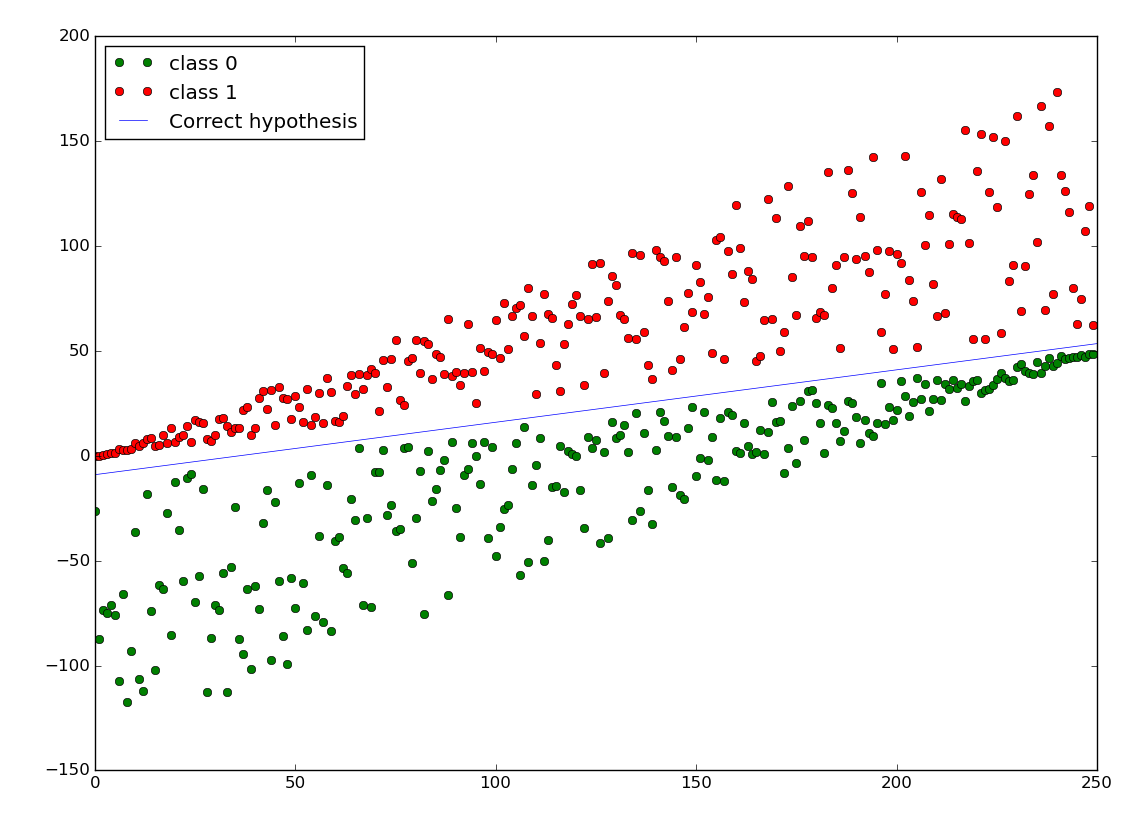
\includegraphics[width=6in,clip,keepaspectratio]{data.png}\
	\caption{Generated data}	
\end{figure}

Then we define a function, that generates random hypotheses in such a fashion that some of them might and would work for some test samples:
\begin{lstlisting}[frame=single]  
def generateH(num):
	H = [[-9 * (random.random() + 0.5)*5, 0.25*(3*random.random() - 0.5)] for i in xrange(num)]
	H.append([-9, 0.25]) #add correct hypothesis
	return H
\end{lstlisting}

Now using Halving algorithm, which defined as following:
\begin{lstlisting}[frame=single]  
def Halving(H, S, verbose=True):
	numMistakes = 0
	for i in S:
		votes = 0
		for h in H:
			votes +=  int(X.x2[i] > h[0] + X.x1[i] * h[1])
		#Derive majority vote
		p = int(votes >= len(H)/2.0)
		numMistakes += int(p <> X.y[i])
		#delete incorrect hypothesis
		[H.remove(h) for h in H if int(X.x2[i] > h[0] + X.x1[i] * h[1]) <> X.y[i]]	
	if verbose:
		print 'h_cap:', H, 'numMistakes: ', numMistakes
	return numMistakes
\end{lstlisting}
	
We test our mistake bound $numMistakes \le log_2(|H|)$ by running the test routing for random test samples (n=0.3 * N) derived from the same distribution (N=500):
\begin{lstlisting}[frame=single]  
def Test(N_RUN, verbose=True):
	mistakes = []
	
	#make 100 runs
	for i in xrange(N_RUN):
		#Define test sample space
		test_i = random.sample(xrange(N), N * 3 / 10)
		H_copy = [h for h in H]		
		#Run Halving algorithm on test sample space and keep numMistakes
		mistakes.append(Halving(H_copy, test_i, False))
	
	if verbose:
		print 'Mistakes: ', mistakes
		print "Mean mistake: %0.2f (sd = %0.2f); Mistake bound: %d; Empirical Risk Bound: %0.2f"
			% (np.mean(mistakes), np.std(mistakes), math.ceil(np.log2(len(H))), 
				np.log2(len(H)/delta)/150)
		return mistakes, np.mean(mistakes), np.std(mistakes)
	return mistakes, np.mean(mistakes), np.std(mistakes)
\end{lstlisting}

To see a dynamic changes in mistake bound we run this routine several times for various set of hypotheses (with various number of them) and take the average:
\begin{lstlisting}[frame=single]  
runs_h = [1, 5, 10, 30, 50, 80]
numMistake_means = []; numMistake_sds = []; mistake_bound = []; emp_risk_bound = []
for i, h_num in enumerate(runs_h):
	H = generateH(h_num)
	mistakes, mean, sd = Test(N_RUN=10)
	
	numMistake_means.append(mean)
	numMistake_sds.append(sd)
	mistake_bound.append(math.ceil(np.log2(len(H))))
	emp_risk_bound.append(np.log2(len(H)/delta)/150)

	plot() #plot the data
\end{lstlisting}

On the figure we can see how good the hypotheses work on average on random samples derived from the same distribution: \pagebreak
     
\begin{figure}[!htb]
	\centering
	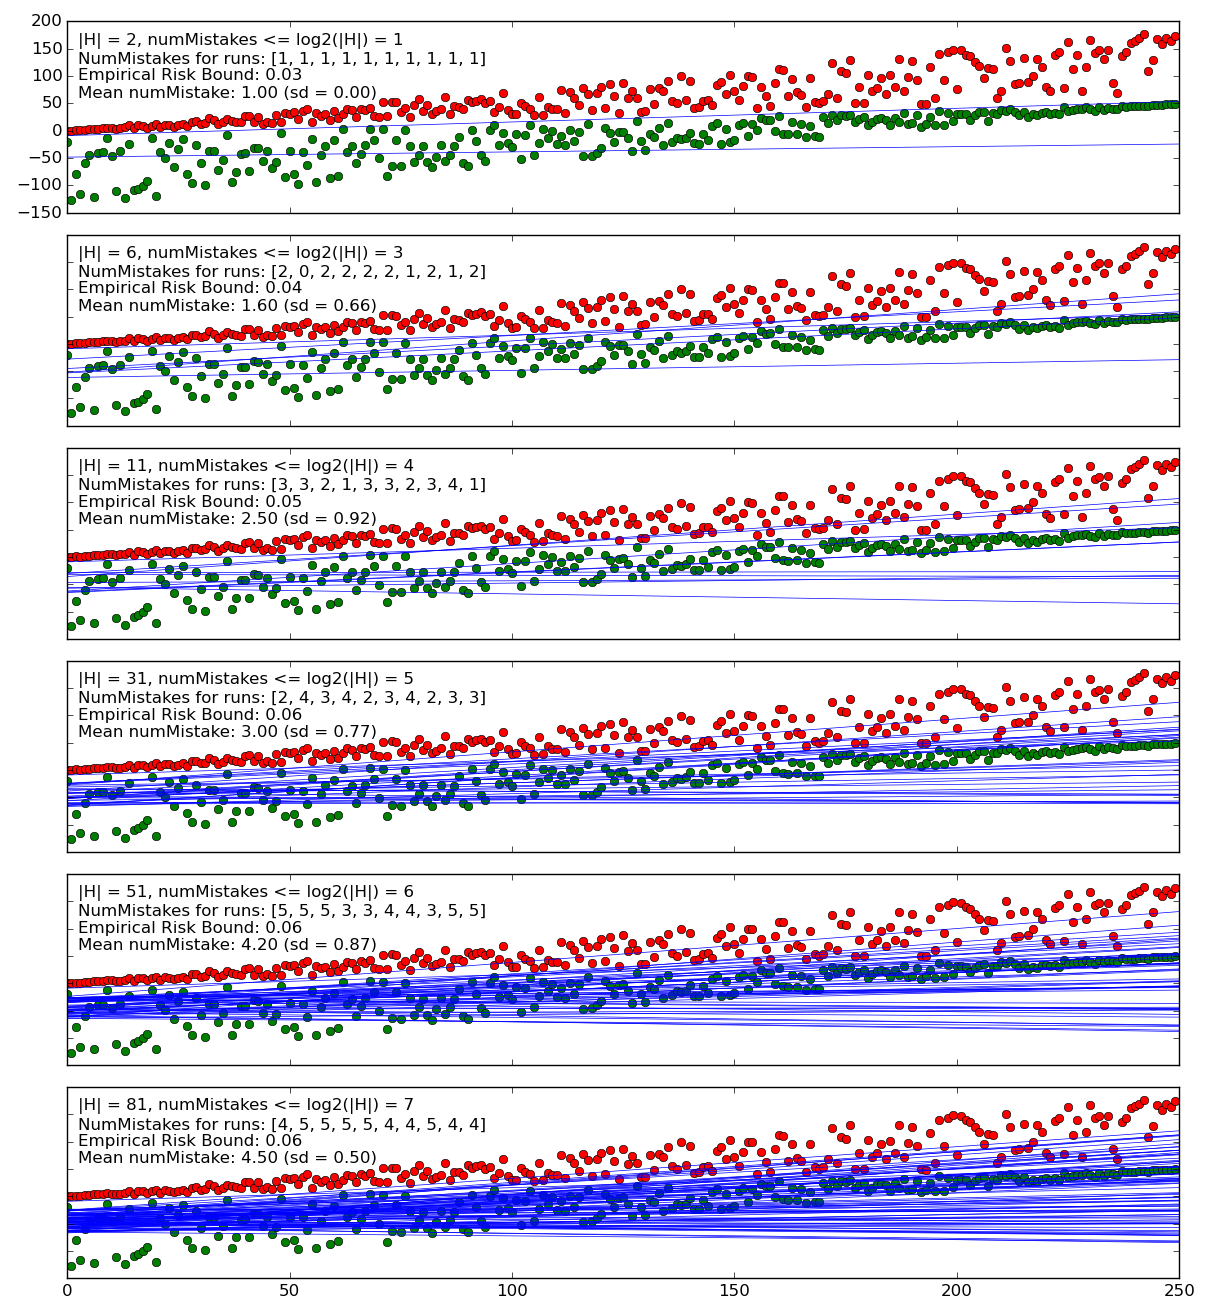
\includegraphics[width=7.2in,clip,keepaspectratio]{mistake_bounds_5runs_v3.png}\
	\caption{Test of "Halving" algorithm for various set of hypotheses}	
\end{figure}     

\pagebreak
Now we can analyze how well our theoretical bound on the number of mistakes $numMistakes \le log_2(|H|)$ correlates with the practical results:
\begin{figure}[!htb]
	\centering
	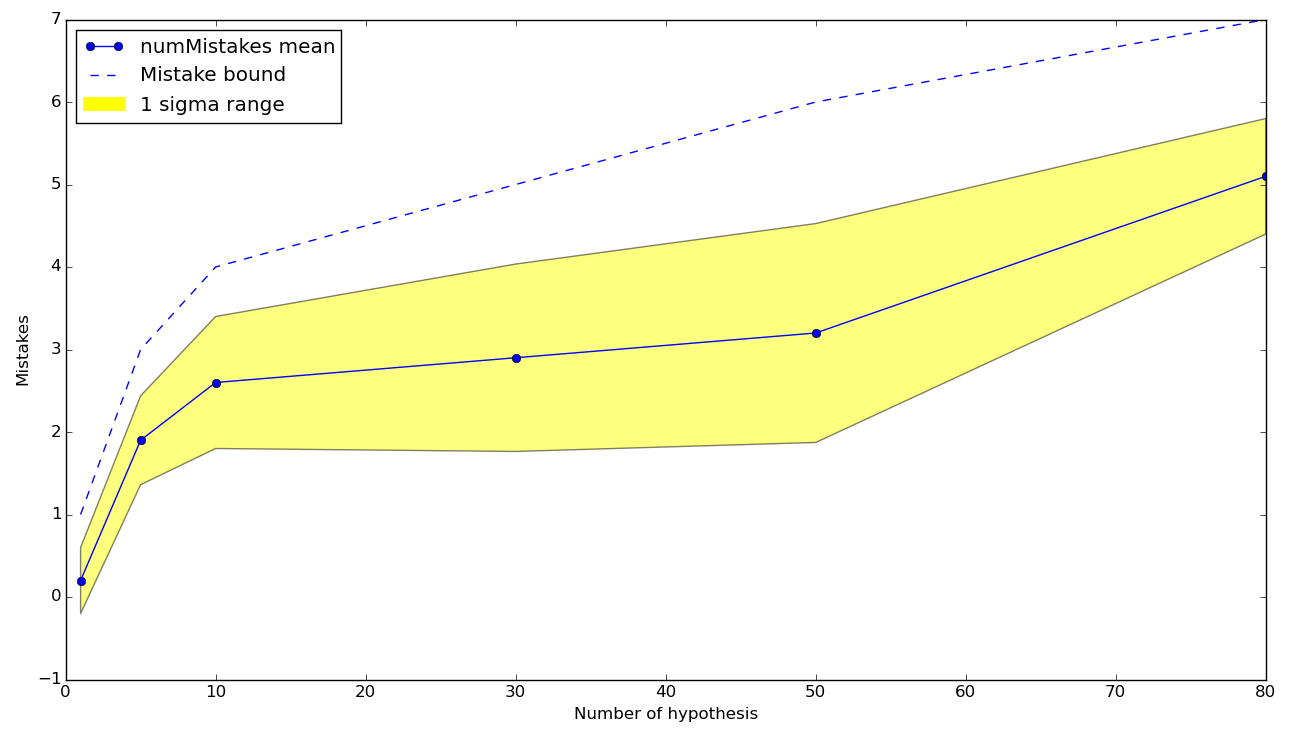
\includegraphics[width=7in,clip,keepaspectratio]{mistake_bounds_5runs_v2_mean_sd_plot.png}\
	\caption{Average number of mistakes as a function of $|H|$}	
\end{figure} 

From figure 3 we can conclude the following:
\begin{enumerate}
	\item Number of mistakes grows with the increase of the set of hypotheses, which is logical. \\
	However, and this is important caveat, \textbf{it does not necessarily does so}. For example, if we generate a million of totally wrong hypotheses - all of them would be rejected at the first step of the Halving algorithm. Thus this increase is only possible, when wrong hypothesis (in a sense, that they do some mistakes on all the examples of the distribution) can perform without mistakes on some subset of examples derived from that distribution.  
	\item As we proven in the section above, number of mistakes could not be more that $log_2(|H|)$, since each time we make a mistake we end up deleting at least a half of the hypotheses. \\
	\textit{Thus our test confirms the analytical bound. }
\end{enumerate}

\pagebreak
We can also plot the empirical risk bound (line is derived as $N * \epsilon (\hat{h})$ )

\begin{figure}[!htb]
	\centering
	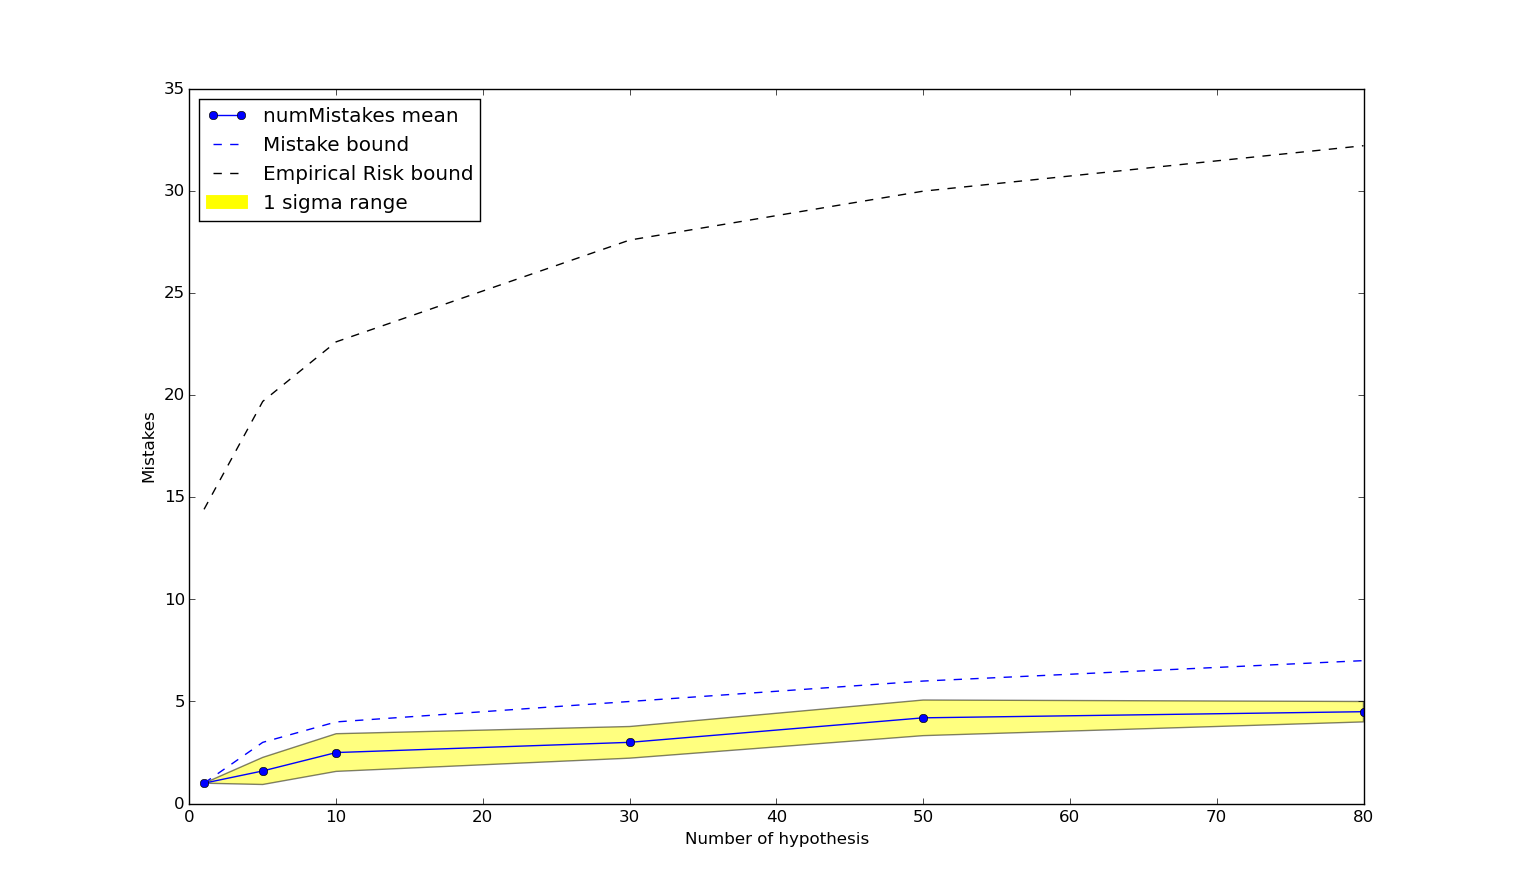
\includegraphics[width=6.4in,clip,keepaspectratio]{emp_risk_bound_w_emp_risk.png}\
	\caption{Empirical risk bound $\epsilon (\hat{h}) \le \frac{1}{m} log \frac{k}{\delta}$ for $\delta=0.1$}	
\end{figure} 
We can clearly see that empirical risk bound is less tight than bound for Halving algorithm. 

Now, what if instead of finite hypotheses set and choosing, we \textbf{did} actually learn? Let us try to learn on subsets with various sizes of all the examples of the given distribution and keep track of how well our optimal (on training data) hypothesis would perform on the entire set of data.

\begin{lstlisting}[frame=single]  
random.seed(123)
RUNS = 10
max_sample_size = 20
sample_start = 1
results = np.zeros([RUNS, max_sample_size - sample_start + 1])
for run in xrange(RUNS):
run_results = []
for size in xrange(sample_start, max_sample_size+1):
	test_i = random.sample(xrange(N/2), size) + random.sample(xrange(N/2, N), size)
	test_X = X.ix[test_i]
	
	#learn the best hypothesis for sample data
	clf = linear_model.LogisticRegression()
	clf.fit(test_X[['x1','x2']], test_X[['y']])
	
	num_mistakes = 0
	#test chosen hypothesis on all the data
	for i in X.index:
	if int(sigmoid(np.dot([X.x1[i], X.x2[i]], clf.coef_.T) + clf.intercept_ ) > 0.5) <> X.y[i]:	
		num_mistakes += 1
		run_results.append(num_mistakes)
		results[run] = run_results
\end{lstlisting}

Again, we see how the empirical risk bound is coherent with our data experiments. 
\begin{figure}[!htb]
	\centering
	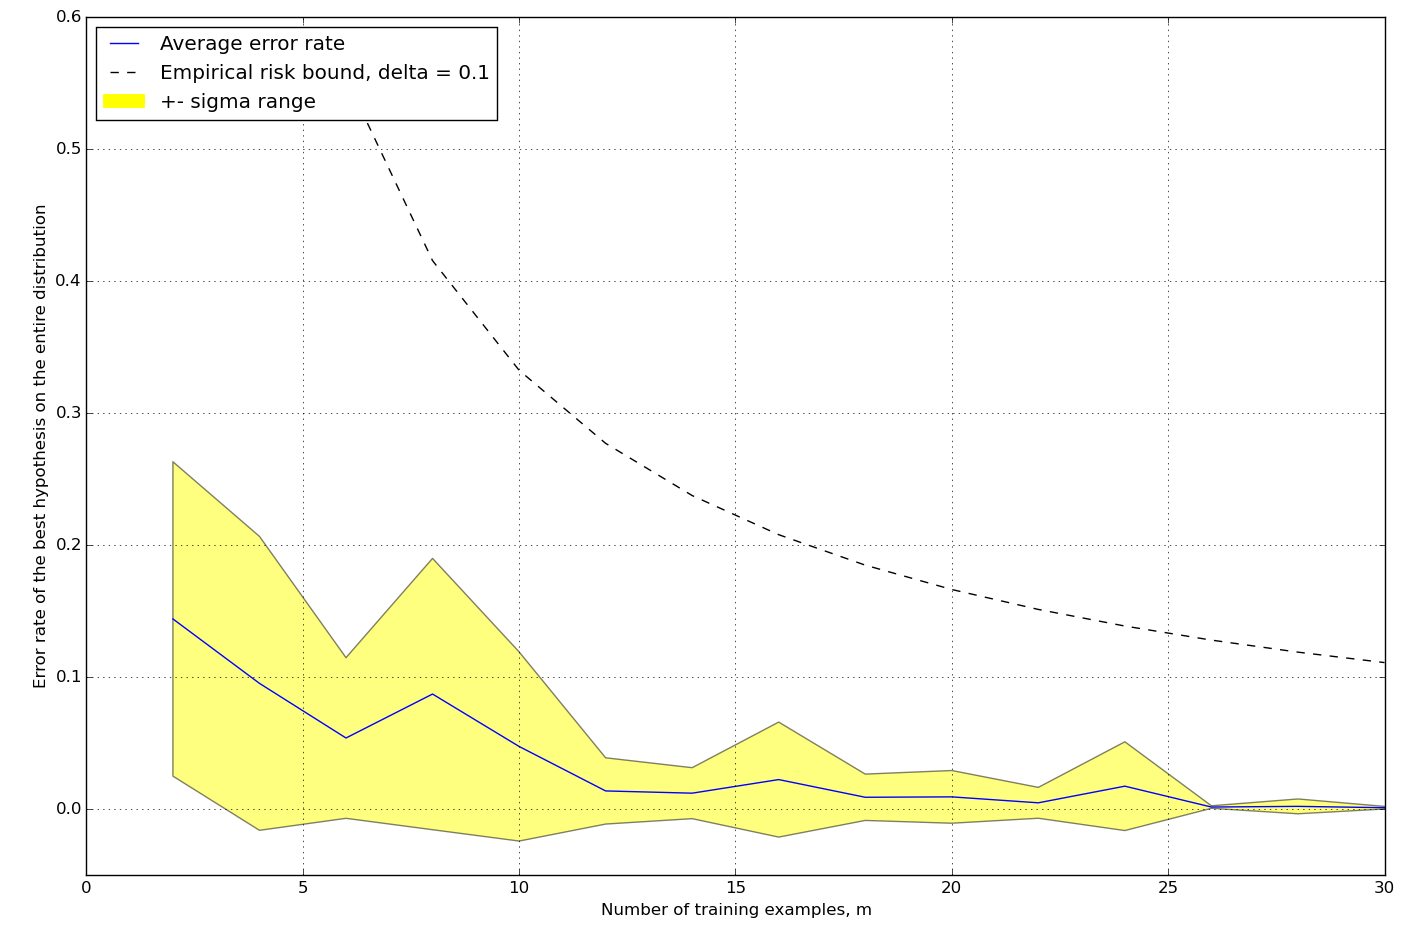
\includegraphics[width=5.5in,clip,keepaspectratio]{emp_risk_bound_v1.png}\
	\caption{Empirical risk bound $\epsilon (\hat{h}) \le \frac{1}{m} log \frac{k}{\delta}$ ($\delta=0.1$) for Linear Regression Classifier}	
\end{figure}
That also holds true for Halving algorithm:
\begin{figure}[!htb]
	\centering
	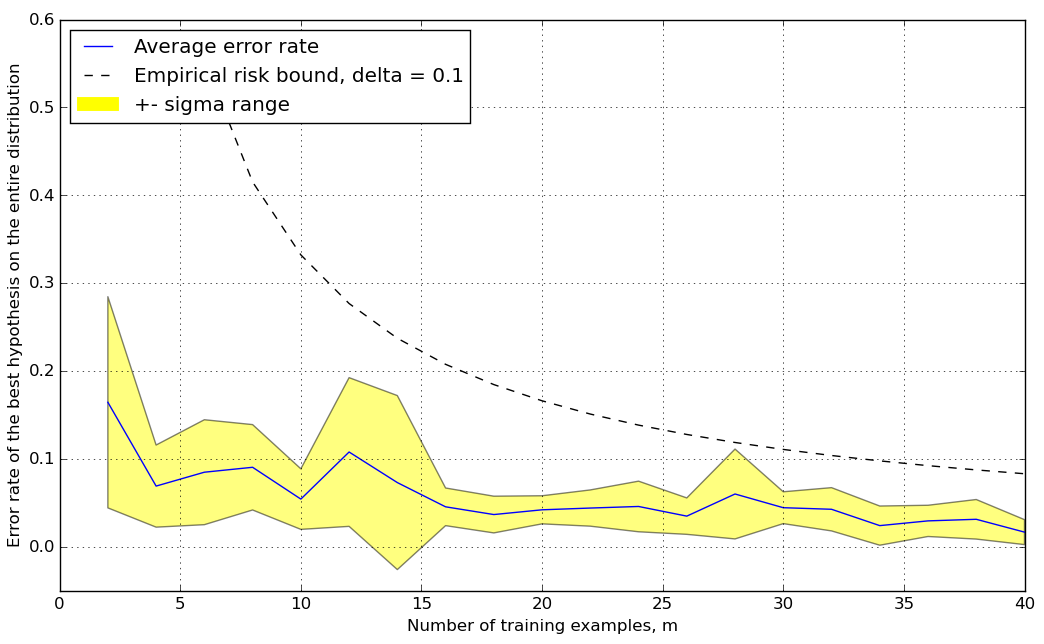
\includegraphics[width=5.5in,clip,keepaspectratio]{emp_risk_bound_finite_H.png}\
	\caption{Empirical risk bound $\epsilon (\hat{h}) \le \frac{1}{m} log \frac{k}{\delta}$ ($\delta=0.1$) for Halving algorithm}	
\end{figure}



\pagebreak
\section{$\ell_2$ norm soft margin SVMs (20 points)}
New algorithm is given by the following optimization problem (notice that the slack penalties are now squared):

$$ \min_{w, b, \xi} \frac{1}{2} ||w||^2 + \frac{C}{2} \sum_{i=1}^{m}\xi_i^2 $$
$$ \text{s.t. } y\ith (w^Tx\ith +b) \ge 1 - \xi_i, i = 1,...,m $$

\begin{itemize}
	\item[(a)] Notice that we have dropped the $\xi_i \ge 0$ constraint in the $\ell_2$ problem. Show that these non-negativity constraints can be removed. That is, show that the optimal value of the objective will be the same whether or not these constraints are present.\\
	\textbf{Proof:}
	\begin{enumerate}
		\item Obviously, the quadratic term of the minimization is indifferent to the negativity of $\xi$ since  $(-a)^2=a^2$.
		\item If $\xi_i \le 0$ then we can set $\xi_i=0$ to satisfy easier the margin constraint $y\ith (w^Tx\ith +b) \ge 1 - \xi_i$  which in turn makes the objective better. Thus, the optimal solution would never get $\xi < 0$ in the first place.  \\
		Explanation: consider related Lagrangian term: 	$-\sum_{i=1}^{m} \alpha_i (y\ith(x^Tw+b)-1 + \xi_i) $. In order to maximize it (given non-positive  $\xi$) we need to use $\xi = 0$.
	\end{enumerate}
	
	
	\item[(b)] What is the Lagrangian of the $\ell_2$ soft margin SVM optimization problem?\\
	\textbf{By definition:}
	$$\mathcal{L}(w,b,\xi,\alpha,r) = \frac{1}{2} ||w||^2 
	+ \frac{C}{2}\sum_{i=1}^{m}\xi_i^2 
	-\sum_{i=1}^{m} \alpha_i (y\ith(x^Tw+b)-1 + \xi_i) $$
	Note, that there is no longer $\sum_{i=1}^{m} \xi_i$ term since we eliminated that constraint.
	
	\item[(c)] Find the critical (minimal) points of the Lagrangian with respect to w, b, and $\xi$ by taking the following gradients: $\nabla_w \mathcal{L}, \frac{\partial \mathcal{L}}{\partial b}, \nabla_\xi \mathcal{L}$,  and setting them equal to 0. Here $\xi = [\xi_1, ..., \xi_m]^T$.
	\begin{align*}
	& \nabla_w \mathcal{L} = w - \sum_{i=1}^{m} \alpha_i y\ith x\ith = 0 
		\rightarrow w = \sum_{i=1}^{m} \alpha_i y\ith x\ith\\
	& \frac{\partial \mathcal{L}}{\partial b} = \sum_{i=1}^{m} \alpha_i y\ith = 0 \\
	& \nabla_\xi \mathcal{L} = C\xi_i - \alpha_i = 0 \rightarrow \xi_i = \alpha_i \frac{1}{C} 
	\end{align*}
	
	
	
	\item[(d)] What is the dual of the $\ell_2$ soft margin SVM optimization problem?
	Let us now plug back derived on the previous step $w, \xi, b$:
	\begin{align*}
	\mathcal{L} &= \frac{1}{2} \sum_{i=1}^{m} \frac{\alpha_i }{\xi_i} \xi_i^2
	+  \frac{1}{2} \sum_{i,j=1}^{m} (\alpha_i y\ith x\ith)^T (\alpha_j y\jth x\jth)
	- \sum_{i=1}^{m} \alpha_i [y\ith((\sum_{j=1}^{m}\alpha_j y\jth x\jth)^T x\ith + b) - 1 + \xi_i]\\	
	&= \frac{1}{2} \sum_{i=1}^{m} \alpha_i \xi_i
	-  \frac{1}{2} \sum_{i,j=1}^{m} \alpha_i \alpha_j y\ith y\jth (x\ith)^T x\jth
	- (\sum_{i=1}^{m} \alpha_i y\ith)b
	+ \sum_{i=1}^{m} \alpha_i
	- \sum_{i=1}^{m} \alpha_i \xi_i \\
	&= \sum_{i=1}^{m} \alpha_i 
	- \frac{1}{2} \sum_{i,j=1}^{m} \alpha_i \alpha_j y\ith y\jth (x\ith)^T x\jth
	- \frac{1}{2} \sum_{i=1}^{m} \frac{\alpha_i^2}{C}
	\end{align*}
	Note that at the last step we used the facts (derived on the \textbf{c} step) that $\sum_{i=1}^{m} \alpha_i y\ith = 0 $ and $\xi_i = \alpha_i \frac{1}{C} $
		
	Thus the dual form:
	$$\max_\alpha \sum_{i=1}^{m} \alpha_i 
	- \sum_{i,j=1}^{m} \alpha_i \alpha_k y\ith y\jth \langle x\ith, x\jth\rangle 
	- \frac{1}{2} \sum_{i=1}^{m} \frac{\alpha_i^2}{C}$$
	\begin{align*}
	\text{s.t. } &\alpha_i \ge 0, i = 1,...,m\\
	& \sum_{i=1}^{m} \alpha_i y\ith = 0 
	\end{align*}
\end{itemize}



\pagebreak
\section{VC dimension (20 points)}
Let the input domain of a learning problem be $\mathcal{X} = \mathbb{R}$. Give the VC dimension for each of the following classes of hypotheses. In each case, if you claim that the VC dimension is d, then you need to show that the hypothesis class can shatter d points, and explain why there are no sets of d + 1 points that it can shatter.

Note, that VC(h) is the size of the largest set shattered by h. H shatters set s if h can realize any labeling on s. In other words, VC dimension is a number of training points that can be classified \textit{exactly}. 
\begin{enumerate}
\item $h(x)=1\{a < x \}$, with parameter $a \in 	\mathbb{R}$\\
With this hypothesis we can shatter any 1 point, but for one particular case of 3 points we \textbf{can't}:\\
\begin{figure}[!htb]
	\centering
	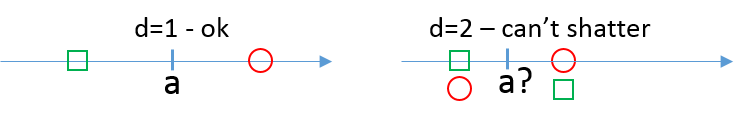
\includegraphics[width=5in,clip,keepaspectratio]{vc_1.png}\
	\caption{VC $h(x)=1\{a < x \}$}	
\end{figure}

That is if we switch the positions of two points we misclassify.
\textbf{Thus, VC(h) = 1}

\item $h(x)=1\{a < x < b\}$, with parameters $a, b \in 	\mathbb{R}$\\
With this hypothesis we can shatter any 2 points, even those we had troubles with previous h, but for one particular pattern of 3 points we \textbf{can't}:\\
\begin{figure}[!htb]
	\centering
	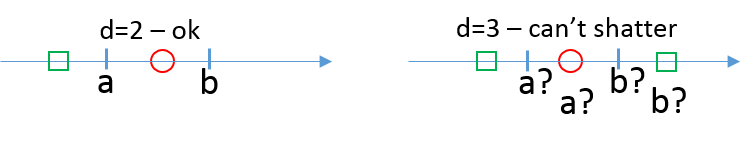
\includegraphics[width=5in,clip,keepaspectratio]{vc_2.png}\
	\caption{VC $h(x)=1\{a < x < b\}$}	
\end{figure}

That is if we for example, have $x_1<x_2<x_3$ and class labels are 1, 0, 1 respectively, then we can't capture both class-1 examples.
\textbf{Thus, VC(h) = 2}

Naturally, if we extrapolate the hypothesis to the extended version:
\begin{displaymath}
	h(x) = \left\{
	\begin{array}{l}
		x < a_1\\
		a_1 < x < a_2\\
		a_2 < x < a_3\\
		...\\
		a_d < x
	\end{array}
	\right.
\end{displaymath}
Then we can clearly see that this hypothesis would shatter any d training points. \\
\textbf{Thus, VC(h) = d}\\

That is, given any sample of points on the line, we can create a sufficient number of intervals to realize any labeling. 

\pagebreak
Obviously enough, there is no upper bound on number of points that could be shattered by sin wave. But the question of the VC dimension is the question of what is the number of examples that sin wave would be able to realize \textbf{any} labeling of them?
\begin{figure}[!htb]
	\centering
	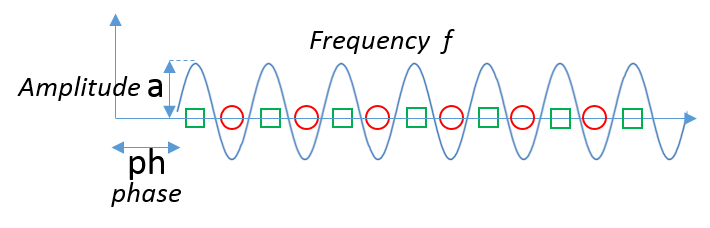
\includegraphics[width=5in,clip,keepaspectratio]{vc_sin.png}\
	\caption{VC for sin weve}	
\end{figure}

\item $h(x)=1\{a sin(x) > 0 \}$, with parameter $a \in 	\mathbb{R}$\\
Be as infinite as it is, sin wave with ability to change it \textbf{amplitude} is useless in shattering even two training points in this case:
\begin{figure}[!htb]
	\centering
	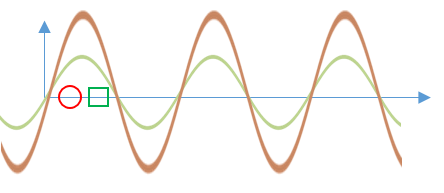
\includegraphics[width=3.6in,clip,keepaspectratio]{vc_3.png}\
	\caption{VC $h(x)=1\{a sin(x) > 0 \}$}	
\end{figure}

\textbf{Thus, VC(h) = 1.}

\item $h(x)=1\{sin(a + x) >0 \}$, with parameters $a \in \mathbb{R}$\\
What about the sin wave with ability to change it \textbf{phase}? It seem like we were able to shatter the previous case, yet more examples make this h stumble. 
\begin{figure}[!htb]
	\centering
	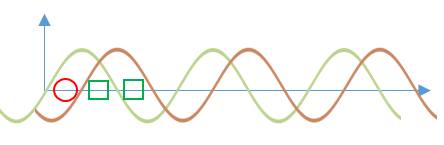
\includegraphics[width=4.5in,clip,keepaspectratio]{vc_4.png}\
	\caption{VC $h(x)=1\{sin(a + x) > 0 \}$}	
\end{figure}

\textbf{Thus, VC(h) = 2.}

\item \textbf{(extra credit)} $h(x)=1\{sin(ax + phase) >0 \}$, with parameters $a \in \mathbb{R}$\\
What about the sin wave with ability to change it \textbf{frequency} and phase? It seems like given sample of points on the line, we can choose a sufficiently large value for frequency and appropriate phase to realize any labeling. That result is similar to the case of large number of intervals for the line. 
\begin{figure}[!htb]
	\centering
	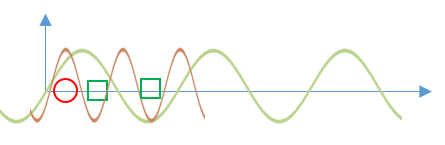
\includegraphics[width=4.5in,clip,keepaspectratio]{vc_5.png}\
	\caption{VC $h(x)=1\{sin(ax + phase) >0 \}$}	
\end{figure}

\textbf{Thus, VC(h) = $\infty$}



\end{enumerate}


 
\end{document}